<<<<<<< HEAD
\documentclass[JohnsonMADraft2.tex]{subfiles}
\begin{document}

\end{document}
\begin{figure}
\centering
\caption{Posterior Means by State}
\label{fig:regimeposteriormeansggplot}
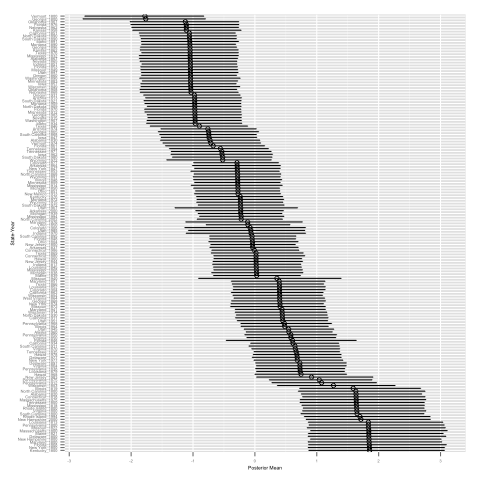
\includegraphics[scale=1.25]{graphics/regimeposteriormeansggplot}
\end{figure}
=======
\documentclass[JohnsonMADraft2]{subfiles}
\begin{document}
I have specified three individual types of models.  A primary specification with four indicators and 200 years of data, an alternative specification with five indicators and 42 years of data, and a regime change specification consisting of regime change observations over 200 years with four indicators.

Each model was run in R using Martyn \citeauthor{rjags}'s JAGS package and the CODA package for convergence diagnostics \cite{R,CODA}.\footnote{Other software packages used are listed in the Reference section without being cited in-text.}\nocite{R,CODA,R-Foreign,R2jags,ggplot2,dplyr,rjags}  Each model was run using 4 chains with 15,000 draws per chain.  The first 10,000 draws were thrown away as burn-in.

\subsection*{Primary Specification}
The primary model is composed of all state year observations between 1800 and 2012.  There are four indicators in this model: Appointment Method, Initial Term Length, Subsequent Term Length and Retention Method.  There are 8436 state-year observations.  

\subsection*{Alternative Specification}
The alternative specification of this model is composed of all state year observations from 1970-2012. There are five indicators in this specification, the same four in the primary specification, with the addition of the indicator for docket control.  

\subsection*{Regime Change Specification}
The final model specification consists of the four original indicators, but is limited to only unique observations of each judicial institution rather than repeated observations over long periods of time.  This specification dramatically reduces the number of observations.  For instance, Massachusetts, which has maintained the same selection/retention methods as well as the same term lengths for its entire history has only a single observation.  There are 155 state-year observations in this model specification.

%\singlespacing
%\bibliographystyle{apsr}
%\bibliography{measurementbib}	
\end{document}
>>>>>>> origin/master
